\chapter{Proyecto: Decisiones de diseño}\label{chap:project} %Materiales y métodos

La finalidad del presente capitulo es explicitar el proceso de investigación y toma de decisiones llevado a cabo durante el proyecto PARKIBIP, mediante los cuales se obtienen los resultados, y por tanto el cumplimiento -parcial o total- de los objetivos establecidos. A partir de las cualidades desafiantes del proyecto, las incertidumbres respecto al contexto clínico y de análisis -marcha de sujetos con EP-, y los objetivos preestablecidos; se optó por conducir durante todo el proyecto una investigación científica, rigurosa, orientada al entendimiento del contexto y a minimizar riesgos -SLR realizada-. De esta manera, todo aquel material, procedimiento o método arbitrario fue descartado mediante un proceso de evaluación de calidad.

\section{Selección tecnológica}\label{seleccion_tecnologica}

En primera instancia y como disparador, se elaboró una revisión de la evidencia científica existente vinculada a los avances tecnológicos y a su aplicación en la detección de las fases de la marcha en personas, con el fin de definir el tipo de dispositivo adecuado a emplear en PARKIBIP (i.e. plantillas inteligentes, unidad de medición inercial, etc.). La misma, se ejecutó en el portal en línea Timbó, el cual habilita a acceder a la última bibliografía y literatura científica-tecnológica mundial reportada.

Para seleccionar la tecnología a utilizar, se consideró una revisión sistemática realizada en el año 2016 \cite{Taborri2016}, la cual identifica, selecciona y categoriza las distintas tecnologías para realizar la detección de las fases del paso, analizando ventajas y desventajas de cada solución. De esta manera, la selección del tipo de sensor se realizó teniendo en cuenta características relevantes para el proyecto en cuestión, entre ellas, el costo, la accesibilidad, la efectividad y la portabilidad del dispositivo.

Bajo los criterios mencionados, el tipo de dispositivo elegido que mejor se adecúa al proyecto fue un dispositivo IMU (del inglés Inertial Measurement Unit o Unidad de Medición Inercial). Estos dispositivos portables, de bajo costo y larga autonomía, han sido utilizados con buenos resultados en el área de análisis de movimientos dinámicos lineales y angulares en los últimos años. Se componen esencialmente de los sensores acelerómetro, giroscopio y magnetómetro, y en ciertos casos se extienden a incluir barómetro, sensores de luz, entre otros.

\section{Estudio de factibilidad} %Metodología de investigación 
Luego de seleccionar el tipo de dispositivo a utilizar, se tomo la decisión de realizar una \textbf{revisión sistemática de la literatura (SLR) respecto al uso de sensores IMU para analizar la marcha de las personas al caminar}. El objetivo de una revisión sistemática es buscar e identificar todo el material relevante relacionado con un tema determinado conforme a responder las preguntas de investigación, siguiendo una metodología objetiva, analítica y tan repetible como sea posible. De acuerdo con los procedimientos descritos en el capítulo de fundamentos, apartado \nameref{fundamentos:RSBE}.

Los principales factores de motivación que impulsaron a aplicar esta metodología fueron:

\begin{itemize}
    \item Adquirir conocimiento respecto a la problemática. Por ejemplo el contexto clínico, el análisis de la marcha y sus fases, la aplicación de sensores IMU y sus desafíos, algoritmos numéricos reportados -matemáticos y computacionales-, entre otros
    \item Corroborar la propiedad innovadora del proyecto -no exista otra que aborde el mismo tema-
    \item Estudiar la marcha de las personas 
    \item Reducir o eliminar incertidumbres en la investigación
    \item Identificar recomendaciones a seguir para PARKIBIP
    \item Identificar las principales metodologías y técnicas aplicadas
\end{itemize}

Si bien elaborar una SLR es un proyecto en sí  mismo, el cual requiere mucho esfuerzo y dedicación, realizarla fue sumamente valiosa y se justifica plenamente tanto con los factores de motivación expuestos como con la obtención de sus resultados en la sección \nameref{synthesis} de la SLR.

El capitulo \nameref{chap_RSBE}, describe el procedimiento completo de la SLR aplicada a la realidad de PARKIBIP, y una variación de sus etapas -de acuerdo al proyecto-. Además, presenta los resultados primarios que responden las preguntas de investigación planificadas, como también los resultados secundarios -no preestablecidos- derivados del análisis pormenorizado del conocimiento relevado.

Bajo el soporte fundamentado de la SLR elaborada, se toman las decisiones pertinentes con el fin de mitigar los riesgos y lograr construir PARKIBIP. Los resultados alcanzados actúan como guía de conclusiones a tomar, algunos puntos son: (i) Proveedores de HW, (ii) Cantidad de dispositivos IMU y ubicación en el cuerpo, (iii) Granularidad de fases a detectar como eventos, (iv) Posibles algoritmos numéricos, (v) Filtro de Orientación eficaz y eficiente.

\section{Benchmark: Elección del dispositivo IMU}\label{section:imu-selection}

Durante el transcurso del estudio de factibilidad y adquisición de conocimiento llevado a cabo mediante la revisión sistemática, se analizaron los distintos proveedores de hardware especializados en soluciones de sensores embebidos. Recordando que, no se encuentra dentro de los objetivos la construcción de una dispositivo de HW -por ende no pertenece al alcance del Proyecto-, fue necesario seleccionar la tecnología (Sec.\ref{seleccion_tecnologica}) a emplear y posteriormente elegir el proveedor de hardware que mejor se adecua a Parkibip.

Existen en el mercado decenas de empresas que ofrecen estos dispositivos junto a sus distintas variaciones, por lo que surgió la necesidad de hacer una evaluación de mercado y elegir la más apropiada. La Tabla comparativa Tab.\ref{tab:imus}  permite visualizar las principales características evaluadas.

\begin{table}[!h]
\caption{Comparación de dispositivos IMU}
\label{tab:imus}
\centering
\hspace*{-3.5cm}%
\begin{tabular}{p{2cm}|p{0.8cm}|p{0.8cm}|p{1cm}|p{1cm}|p{1cm}|p{1cm}|p{1cm}|p{1.2cm}|p{1cm}|p{1cm}|p{1cm}|p{0.8cm}}
 & Arion & BTS G-Sensor & EXL S3 & Inven- Sense & Isen & MMR & Opal APDM Inc & Reha- Gait (HASOMED) & Senno- Gait SmartInsolesPRO & Shim- mer Sensor & Wave- share & Xsens   \\ \hline
Acelerómetro (3-axis) & SI & SI & SI & SI & SI & SI & SI & SI & SI & SI & SI & SI \\ \hline
Giroscopio (3-axis) & SI & SI & SI & SI & SI & SI & SI & SI & SI & SI & SI & SI \\\hline
Magnetómetro (3-axis) & NO & SI & SI & SI & SI & SI & SI & SI & SI & SI & SI & SI \\ \hline
Barómetro & SI & NO & NO & NO & SI & SI & NO & - & NO & NO & SI & NO \\ \hline
Altímetro & - & - & - & NO & NO & SI & - & - & NO & SI & NO & NO \\ \hline
Bluetooth & SI & SI (3.0) & SI (2.1) & NO (I2C, SPI) & NO & SI (LE) & NO & SI & SI & SI & NO & - \\ \hline
Wifi & NO & NO & NO & NO & SI & NO & NO & NO & SI & NO & NO & NO \\ \hline
Tiempo Real & SI & SI & SI & SI & SI & SI & \textless 30ms & - & - & - &  & \textless 2 ms \\ \hline
Runtime calibration & NO & NO & NO & SI & SI & SI & - & - & - & SI &  & - \\ \hline
Peso & - & 37gr & 22g & - & 46g & 8.5 g & \textless 25g & - & - & 23.6g & 3g & - \\ \hline
Medidas (mm) & - & 70 x40 x18 & 54 x33 x14 & 3 x3 x0.9 & 56 x38 x18 & 24 x17 x4 & 43 x39 x13 & 60 ×15 ×35 & 35-45 & 51 x34 x14 & 31 x16 x2.5 & 57 \\ \hline
Batería & $\sim$7hs & $\sim$8hs & 2 hs & - & $\sim$3.5 hs & 2-14d & 8-16hrs & - & \textgreater{}48hrs & - & - & - \\ \hline
SDK Android & NO & NO & NO & SI & SI & SI & No & NO & NO & SI &  & SI \\ \hline
SDK iOS & NO & NO & NO & NO & NO & SI & No & NO & NO & NO &  & NO \\ \hline
Comunidad OpenSource & NO & NO & NO & SI & NO & SI & NO & NO & NO & NO &  & NO \\\hline
Documenta-ción & NO & NO & NO & SI & NO & SI & NO & NO & NO & SI &  & SI \\ \hline
Vibración & NO & NO & NO & NO & NO & SI & NO & NO & NO & NO &  & NO \\ \hline
Precio & \euro 189 & - & - & - & - & USD99 & - & - & - & \euro 359 & USD16 & \euro 800 \\ \hline
\end{tabular}
\hspace*{-3.5cm}%
\end{table}

%Dispositivos, sensores usados
A efecto de la etapa, se concluyó en la utilización de la solución de producto de dispositivos vestibles MetaMotionR (MMR). Además de ser un dispositivo liviano, accesible y de bajo costo; integra los principales sensores de lectura, como lo son el acelerómetro (BMI160 6-Ejes), el giroscopio (BMI160 6-Ejes), el magnetómetro y la unidad vibratoria. 

\section{Cantidad y ubicación del dispositivo}

Se cree pertinente emplear dos dispositivos IMU sincronizados, unidos con bandas elásticas de velcro a los tobillos -justo por encima de los maléolos- de los pacientes con la enfermedad de Parkinson tal como indica la Fig. \ref{FIG:foot_strap}. De esta manera, es posible estudiar el comportamiento y las distintas variables vinculadas a cada extremidad por separado, así como combinarlas para lograr otros resultados genéricos. De forma complementaria, la decisión logra un espectro o visión de análisis mas amplio, el cual habilita a escalar el alcance del proyecto en materia de variables de la marcha o patologías (i.e. rotaciones, asimetrías, etc.).

\begin{figure}[h!]
\centering
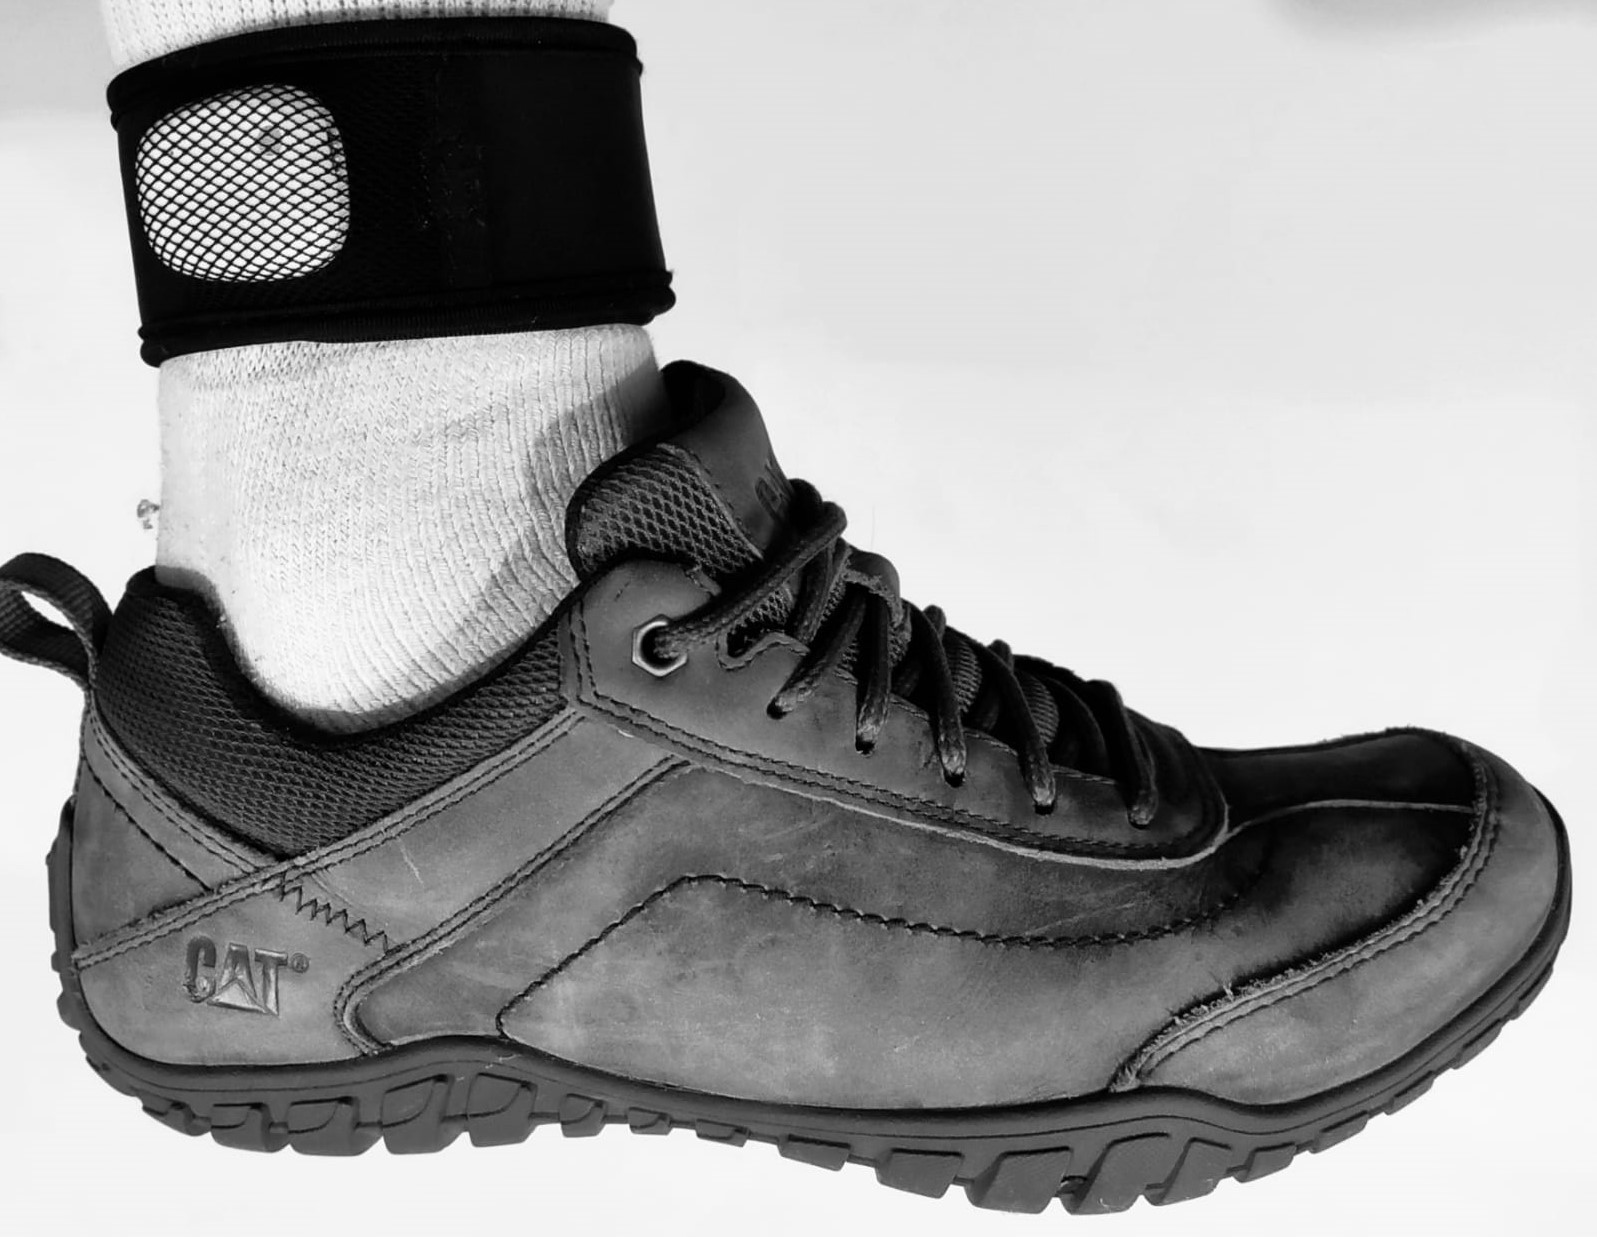
\includegraphics[clip,width=0.78\columnwidth]{TESIS/imagenes/img/footstrap.jpeg}
\caption{Banda elástica junto a la unidad de medición inercial (IMU).}
\label{FIG:foot_strap}
\end{figure}

\section{Granularidad de fases de la marcha} \label{section:partition-cycle}

%Fases de la marcha y las que vamos a identificar.
Estandarizando los conceptos de fases de la marcha, tal como se sintetiza en \cite{Taborri2016}, se pueden emplear distintas granularidades de las fases de la marcha (i.e. dos, tres, cuatro, cinco, seis, siete y ocho), tal como indica la Fig. \ref{FIG: ciclo}.

\begin{figure}[h!]
\centering
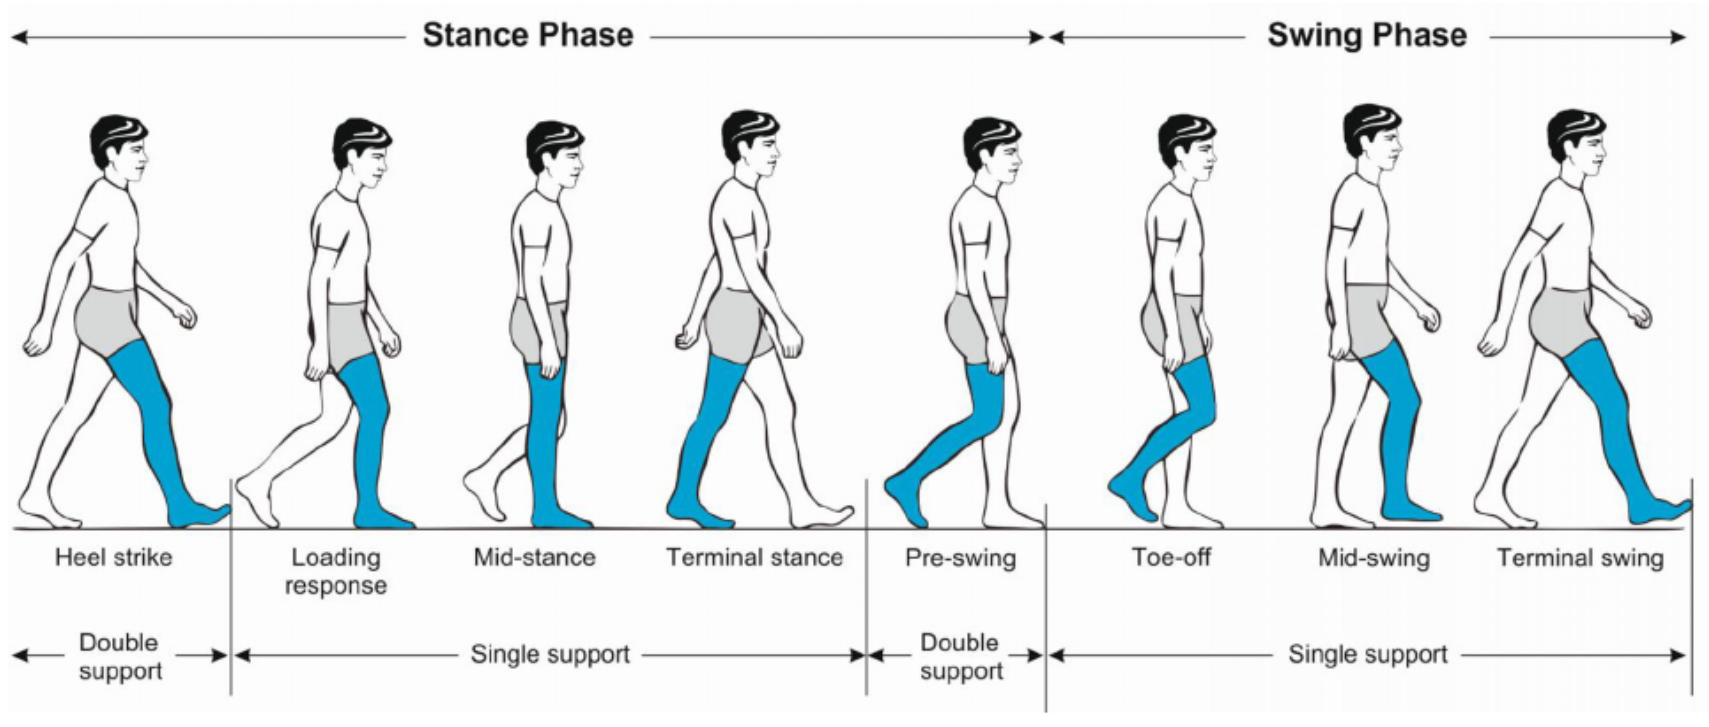
\includegraphics[clip,width=1.05 \columnwidth]{TESIS/imagenes/img/gaitcycle.png}
\caption{Partición del ciclo de la marcha normal en 8 fases. Tomado de ``W. Pirker y R. Katzenschlager'' \cite{Pirker2016}.}
\label{FIG: ciclo}
\end{figure}

El presente proyecto reconoce dos fases en el ciclo de la marcha, fase de apoyo y fase vuelo. En este sentido, los algoritmos matemáticos considerados se enfocan en detectar eficazmente los eventos golpe de talón (HS, del ingles Heel Strike) y el despegue de los dedos del pie (TO, del ingles Toe Off).

\section{Filtro de Orientación}\label{section:filter_orientation}

%1. Objetivo del filtro
La estimación precisa de la orientación de un cuerpo desempeña un rol critico en una variedad de campos: aeroespacial, robótica, navegación y análisis del movimiento humano e interacción de máquinas. Por ejemplo, en la estimación de las fases de la marcha y el cálculo de parámetros espacio-temporales. Si bien una variedad de tecnologías permiten la medición de la orientación, los sistemas inerciales presentan la ventaja de ser completamente autónomos, de modo que la entidad de medición no está restringida ni en movimiento, ni a ningún entorno o ubicación específicos.

La función de un filtro de orientación es calcular una única estimación de orientación de un cuerpo relativo a un marco de referencia inercial; a través de la fusión óptima del giroscopio, acelerómetro y magnetómetro. 

%2. Errores propagados, etc.
La principal limitante para el computo de la orientación es el error propagado a algoritmos al estimar la orientación. Para un mayor entendimiento, se mencionan ciertos inconvenientes: 
\begin{itemize}
    \item Un acelerómetro y un magnetómetro medirán los campos gravitacionales y magnéticos de la tierra, y proporcionarán una referencia absoluta de orientación. Sin embargo, es probable que estén sujetos a altos niveles de ruido (i.e. las aceleraciones debidas al movimiento corromperán la dirección de la gravedad medida). La integración doble de datos de aceleración, por ejemplo, daría como resultado cantidades muy elevadas de error residual, ya que la deriva se acumularía cuadráticamente.
    \item Un giroscopio (velocidades angulares) requiere conocer condiciones iniciales, y puede integrarse en el tiempo para calcular la orientación del sensor. La integración de los errores de medición del giroscopio conducirán a un error acumulado en la orientación calculada. Por lo tanto, los giroscopios por sí solos no pueden proporcionar una medida absoluta de orientación.
    \item Ciertos métodos requieren alta complejidad computacional o en otros casos no se pueden implementar. Adicional, pueden demandar frecuencias de muestreos de datos que superen el ancho de banda; por ejemplo, una frecuencia de muestreo entre 512 Hz y 30 kHz.
\end{itemize}

El problema se incrementa cuando deseamos calcular parámetros espacio-temporales, las estimaciones de posición y velocidad basadas en acelerómetros de sensores de bajo costo (IMU) son muy malas e inutilizables. Esto no se debe a que los acelerómetros en sí sean deficientes, sino a que la orientación del sensor debe conocerse con un alto grado de precisión para que las mediciones de gravedad se puedan distinguir de la aceleración física del sensor. Incluso pequeños errores en la estimación de la orientación producirán errores extremadamente altos en la aceleración medida, lo que se traduce en errores aún mayores en las estimaciones de velocidad y posición.

% Importancia
Por lo tanto, estimar la orientación de un cuerpo resulta en un verdadero desafió computacional y un cuello de botella en los sistemas de análisis de la marcha (alta dependencia en algoritmos). Sin embargo, es una necesidad para PARKIBIP, y se debe emplear un algoritmo eficaz y eficiente que se ajuste a la propuesta del presente proyecto, convirtiéndolo en un desafío aun mayor. Un algoritmo lento y costoso conllevará a retardos en las estimaciones de las fases de la marcha (por ende los estímulos asociados) y a consumos excesivos de los recursos del dispositivo inteligente (desgaste energético y rendimiento del dispositivo). 
 
%3.Otros métodos de Orientación: Mahony y rotaciones estáticas.
Los sistemas denominados \gls{AHRS} (por sus siglas en inglés, Attitude and Heading Reference Systems) pueden proporcionar una medición completa de la orientación relativa a la dirección de la gravedad y el campo magnético de la tierra. Existen diversas técnicas que logran buenas aproximaciones y fueron excelentes resultados -inputs para el presente hito- de la \nameref{chap_RSBE} para identificar el filtro de orientación a emplear. La construcción de matrices de rotación en base a los ángulos de Euler, el método sugerido por Martin \& Salaun \cite{Martin2010}, la técnica propuesta por Mahony \cite{Mahony2006} y el filtro propuesto por S. Madgwick \cite{Madgwick}.

Para el caso Mahony (muy empleado), combina las señales crudas del acelerómetro y el giroscopio mediante el uso de un algoritmo de estimación de orientación propuesto. Para eliminar la deriva del giroscopio y proporcionar la orientación del sensor en el espacio, se emplea un vector de corrección a partir de la orientación  estimada previamente y el vector acelerómetro instantáneo. En cambio, la implementación de S. Madwick incorpora la distorsión magnética (combinando el magnetómetro) y la compensación de deriva del giroscopio; reportándose en la literatura mejores resultados con éste ultimo método. 

%5.Método a emplear
A su vez, Madwick proporciona ciertos beneficios adicionales: (i) computacionalmente económico; requiriendo 109 (IMU) o 277 (MARG) operaciones aritméticas escalares cada actualización de filtro, (ii) efectivo a bajas tasas de muestreo; p.ej. 10 Hz y (iii) contiene 1 (IMU) o 2 (MARG) parámetros ajustables a definir por las características del sistema. Por consiguiente, para estimar la orientación de los dispositivos, se decide aplicar la técnica de gradiente descendiente optimizado y derivado analíticamente sugerida por Madgwick, descripta en la FIG. \ref{FIG: madgwick} tomada de \cite{Madgwick}.

\section{Detección de Velocidad Cero}

Los dispositivos inerciales de bajo costo sufren de deriva en sus sensores, debido a la naturaleza integradora de los sistemas de navegación inercial (INS), cualquier desviación pequeña se acumulará y crecerá con el tiempo sin límites. Este suceso genera un error en la estimación de la posición, que crece proporcionalmente al cubo del tiempo de operación del sistema. De este modo, la navegación inercial solo es factible durante períodos de tiempo en el rango de unos pocos segundos. Sin embargo, el crecimiento del error cúbico puede reducirse imponiendo restricciones en la solución sobre la dinámica del sistema de navegación inercial \cite{Isaac2009}.

En general, un tipo de información utilizado para este propósito es la detección de los intervalos de tiempo en los cuales el sistema está en una fase estacionaria, es decir, cuando el sistema tiene una posición y una orientación constante. Este método se lo conoce como ZUPT (por sus siglas en inglés). El uso de actualizaciones de velocidad cero es especialmente atractivo para reducir el error en los INS que se encuentran montados a los pies del sujeto, ya que durante el ciclo de la marcha el pie vuelve a un estado estacionario. La figura Fig. \ref{fig:zero-velocity} permite visualizar un flujo del proceso -enfocado en \gls{ZVD} (del inglés Zero Velocity Detector) y abstrayendo otros componentes- empleado en PARKIBIP.

\begin{figure}[H]
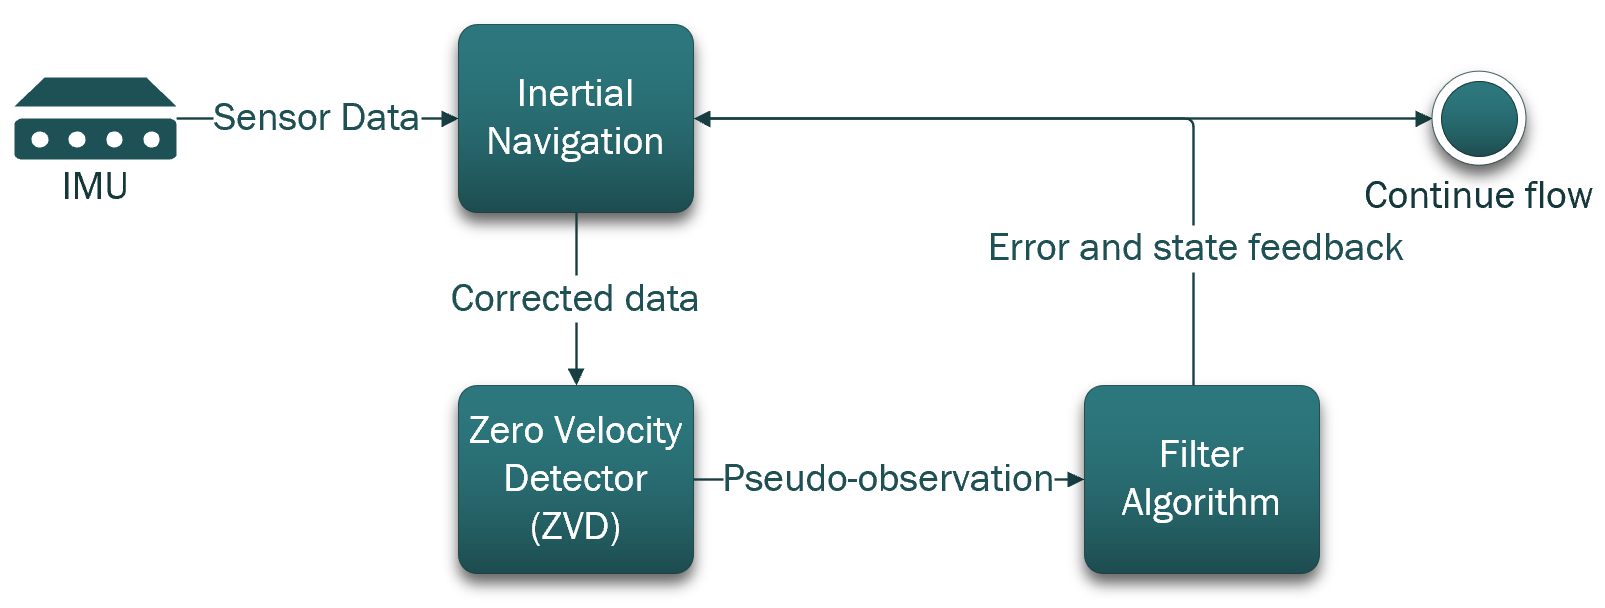
\includegraphics[width=\textwidth]{TESIS/imagenes/chap04/zero-velocity.PNG}
\caption{ Flujo de detección de velocidad cero (ZVD) de PARKIBIP.}
\label{fig:zero-velocity}
\end{figure}

\noindent Cuando el ZVD decide que el IMU se encuentra estacionario, el sistema genera una pseudo-observación y emite un evento hacia el algoritmo de filtrado del detector. El filtro compara la pseudo-observación con la estimación de velocidad del INS y usa la diferencia para estimar los errores del INS. Las estimaciones de error se retroalimentan para reducir el error acumulativo.

Luego, detectados los momentos de cero velocidad, es trivial inferir que los algoritmos ZVD´s permiten reconocer las transiciones de fases dentro del ciclo de la marcha. Por ejemplo, un ciclo binario Stance|Swing -fases de apoyo y vuelo-.

El problema de identificar los instantes de velocidad cero se formaliza como un problema de test binario de hipótesis -$H_0:$ hipótesis nula, $H_1:$ hipótesis alternativa-, y se analiza aplicando la teoría de detección estadística. Algunos ejemplos de algoritmos de ZVD son: (i) Acceleration moving variance detector -MV-, (ii) Acceleration magnitude detector -MAG-, (iii) Angular rate energy  detector (ARE), Generalized Likelihood Ratio Test -GLRT-, entre otros.

Por lo tanto, se propone la utilización de algoritmos de ZVD para romper la deriva del error cúbico mediante la técnica de ZUPT e inferir el ciclo de la marcha del sujeto en deambulación. Además, se enfatiza en el requerimiento online del sistema PARKIBIP, acentuando la complejidad de la solución. Para ello, se construirá una combinación estandarizada de algoritmos óptimos en su función (e.g. Kalman Filter, Orientation Filter, ZVD, otros algoritmos auxiliares), cuya sinergia incremente la operativa de PARKIBIP y habilite a cumplir los propósitos de dicho INS.

\section{Filtro de Kalman}\label{section:kalman-filter}

Un método de filtrado lineal de gran utilidad y con variadas aplicaciones, es el \gls{kalman-filter} (KF, por sus siglas en inglés) en sus diversas variedades. En estadística y teoría de control, el KF, también conocido como estimación cuadrática lineal (LQE), es un algoritmo que utiliza una serie de mediciones observadas a lo largo del tiempo -que contienen ruido estadístico y otras inexactitudes-, y produce estimaciones de variables desconocidas que tienden a ser más precisas que los basados en una sola medición. Suponiendo fuentes de ruido distribuidas como variables aleatorias gaussianas, el filtro de Kalman proporciona la solución que minimiza el error cuadrático medio (MMSE) del problema lineal pre-establecido.

En otras palabras, KF es un algoritmo óptimo de estimación que permite hallar la mejor estimación de variables de interés -no medibles- a partir de la combinación de variables indirectas -medibles-. De esta manera, se logra extraer información respecto a algo que no es posible medir, desde algo que si lo es.

Con la finalidad de introducir a la temática se mencionan brevemente algunas de sus aplicaciones. Los filtros de Kalman o su variación extendida para sistemas no lineales, son de gran utilidad en la robótica dado que facilitan el problema de la planificación de un camino mínimo. Un clásico problema de la navegación robótica que puede ser resuelto con dicho algoritmo, es planificar el movimiento de un robot que viaja con una velocidad limitada, desde un determinado punto a otro en una superficie en presencia de obstáculos en movimiento \cite{Nasir2017}.
\noindent Otra aplicación es lo que se denomina control y navegación de vehículos, en particular aviones, naves espaciales y barcos posicionados dinámicamente \cite{Mao2007}. Además, KF es un concepto ampliamente aplicado en el análisis de series de tiempo que se utiliza en campos como el procesamiento de señales y la econometría.

Para entrar en contexto con la utilidad de KF en PARKIBIP, se expone el problema de un sistema de navegación de un automóvil en movimiento, al estimar la posición del mismo dentro de un túnel. El automóvil integra dispositivos de medición a bordo, como lo son un IMU (acelerómetro y giroscopio) y un GPS (estima la posición en base a señales satélitales).
\noindent Dentro del túnel, el sensor de GPS se ve afectado por el bloqueo de señal satélital (e.g. señal intermitente y de baja frecuencia, ruido en el receptor). Análogamente, realizar la doble integración de la señal del acelerómetro recibida desde el IMU -para obtener la posición-, se encuentra sujeta a desvíos incrementales debido al error acumulativo de integración respecto al tiempo. 
\noindent Por lo tanto, los dispositivos de medición a bordo no logran estimar la posición por si solos. En éste escenario, un KF puede ser usado para fusionar las mediciones de los sensores y hallar la solución óptima al problema de estimar la posición del vehículo en su sistema de navegación.

\begin{figure}[H]
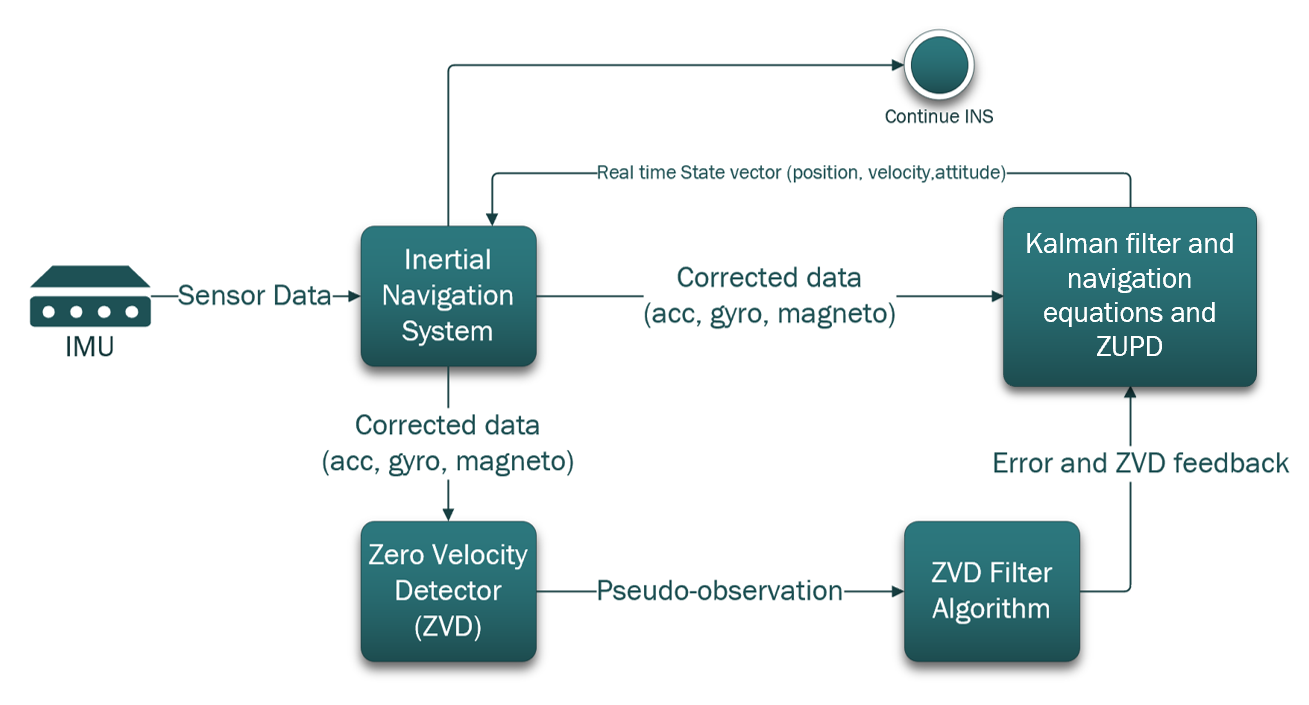
\includegraphics[width=\textwidth]{TESIS/imagenes/chap04/zero-velocity-kalman.PNG}
\caption{ Flujo de filtro de Kalman para estimar las variables indirectas posición, velocidad, altitud de un IMU en movimiento en PARKIBIP. Además, integra la compensación de actualizaciones de velocidad cero (ZUPD) mediante la fusión de un algoritmo de detección de velocidad cero (ZVD).}
\label{fig:zero-velocity-kalman}
\end{figure}

En estas condiciones, PARKIBIP empleará el filtro de Kalman para predecir en tiempo real las variables indirectas velocidad, posición y altitud (variables no medibles por un IMU) a partir de las mediciones de acelerómetro, giroscopio y magnetómetro. Asimismo, otra entrada al algoritmo, serán los momentos de cero velocidad detectados por el algoritmo de ZVD, que permitirán aplicar el ZUPT dentro del filtro de Kalman para compensar y mejorar aun mas la solución de navegación. El filtro de Kalman no solo estima el error de velocidad en los intervalos ZUPT detectados, sino que también estima las correcciones de posición, altitud, y ruido de los sensores inerciales debido a correlaciones cruzadas en la matriz de transición. La figura Fig. \ref{fig:zero-velocity-kalman} brinda un modelo de flujo de aplicación que integra los conceptos mencionados.

\section{Desarrollo de una aplicación móvil PARKIBIP}

Dentro de las expectativas funcionales del proyecto PARKIBIP se encuentra la de brindar una herramienta tecnológica que le permita a los pacientes con la enfermedad de Parkinson una rehabilitación personal; que en la actualidad es inexistente. Asimismo, se espera que dicha herramienta sea un soporte para el terapeuta al momento de tomar decisiones y evaluar al sujeto afectado. De esta manera, se logra una evaluación clínica mas objetiva, que de otra forma se hace dificultosa debido a una serie de limitaciones estructurales, logísticas y financieras.

En la actualidad, los sistemas de análisis de movimiento ópticos basados en cámaras (3D-GA) son reconocidos como el estándar de oro en la medición del movimiento. Sin embargo, requieren ejecutar las pruebas en un entorno de laboratorio con equipos de alto costo, solo se pueden usar para evaluar segmentos cortos de la marcha, requiere personal especializado, equipo considerable -i.e. laboratorio de marcha-, tiempo y sobretodo una gran inversión.

Por consiguiente, se quiere implementar un instrumento portable, accesible y de bajo costo; cuyo usuario final sea un Terapeuta y/o un Parkinsoniano. Primero, mencionado en la sección \nameref{seleccion_tecnologica}, se optó por un dispositivo que cumpla los requerimientos antedichos y sea de gran amigabilidad para su portador (i.e. pequeño, cómodo, portable). Luego, se requiere un elemento de hardware que permita interoperar con el dispositivo, procesar información y presentar resultados al usuario. 

En la actualidad, prácticamente todas las personas cuentan con dispositivos inteligentes personales con los cuales interactúan todo el día en sus tareas cotidianas. Aquí, es donde nace una gran oportunidad para PARKIBIP de combinar la tecnología IMU con los teléfonos inteligentes, aprovechando todo su potencial:

\begin{itemize}
    \item Permite una comunicación directa y personalizada hacia el usuario
    \item Ofrece atención continua (i.e. apps están disponibles 24x7)
    \item Usabilidad. Es una tecnología conocida, el desafío central es la amigabilidad en el diseño hacia el usuario.
    \item Acceso a periféricos del dispositivo. Por ejemplo el Bluetooth, requisito para enlazar a un IMU
    \item Dispositivo de procesamiento (variando el rendimiento según las características del mismo) 
\end{itemize}

Finalmente, en consideración de las necesidades de PARKIBIP y los beneficios mencionados, se propone la implementación de una aplicación móvil adecuada para el usuario final (conceptos como usabilidad, rendimiento y automatización).

\newpage

\section{Sistema operativo y lenguaje utilizado}

% Android 
La implementación del Software PARKIBIP consistió principalmente en el desarrollo de una aplicación móvil. Una decisión clave para el proyecto fue decidir el sistema operativo a emplear, en el cual se desarrolló esta aplicación. Según la herramienta StatCounter (© 1999-2020 StatCounter), la cual permite consultar estadísticas globales sobre el uso de dispositivos móviles, los dos sistemas operativos dominantes en la industria son Android (70.68\%) y iOS (28.79\%), sumando un total del 99.47\% del mercado entre estas dos plataformas.

\begin{figure}[H]
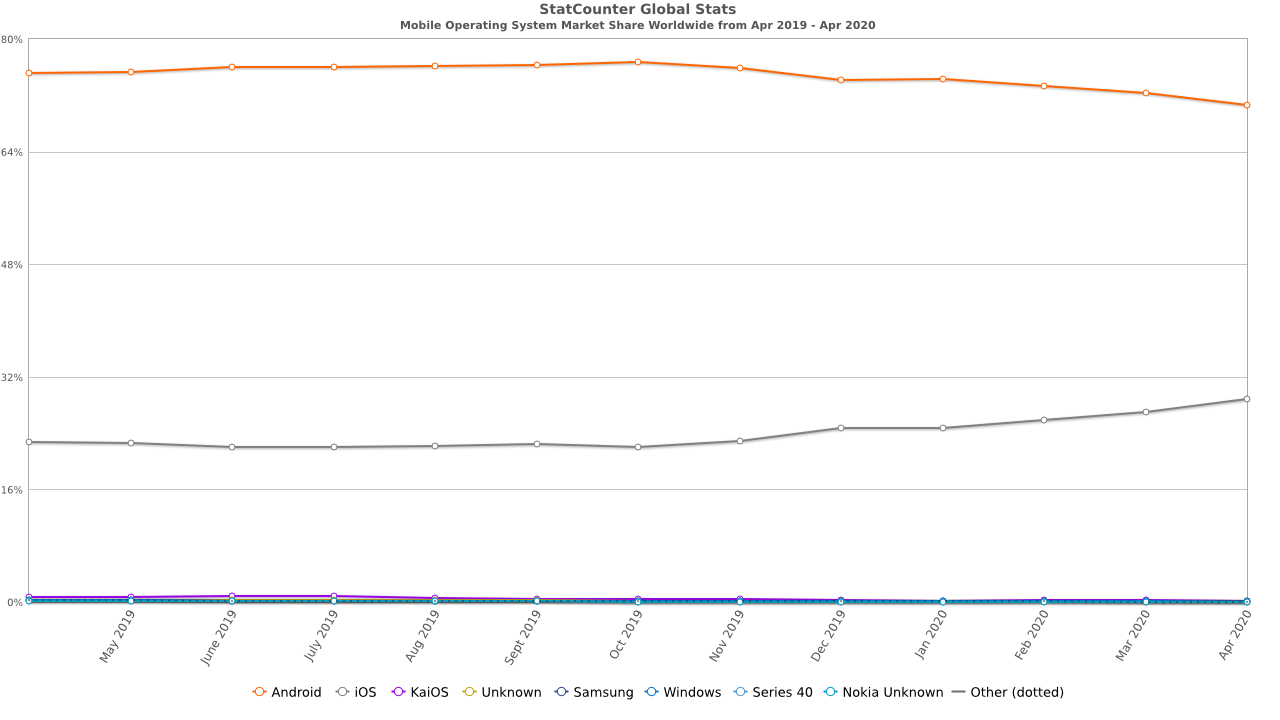
\includegraphics[width=\textwidth]{TESIS/imagenes/chap04/StatCounter-os_combined-ww-monthly-201904-202004.png}
\caption{ Evolución global de sistemas operativos en dispositivos móviles desde 04.2019 a 04.2020 \cite{StatCounter} }
\label{fig:ww-mobile-so}
\end{figure}

Uruguay no es la excepción, en donde Android es aún más dominante con respecto al resto de los sistemas operativos. En la figura Fig. \ref{fig:uy-mobile-so} se puede observar que el 85.41\% de los dispositivos móviles de Uruguay contienen un sistema operativo Android, tan solo un 14.39\% utiliza el sistema iOS y un 0.02\% ejecuta uno diferente. 

\begin{figure}[H]
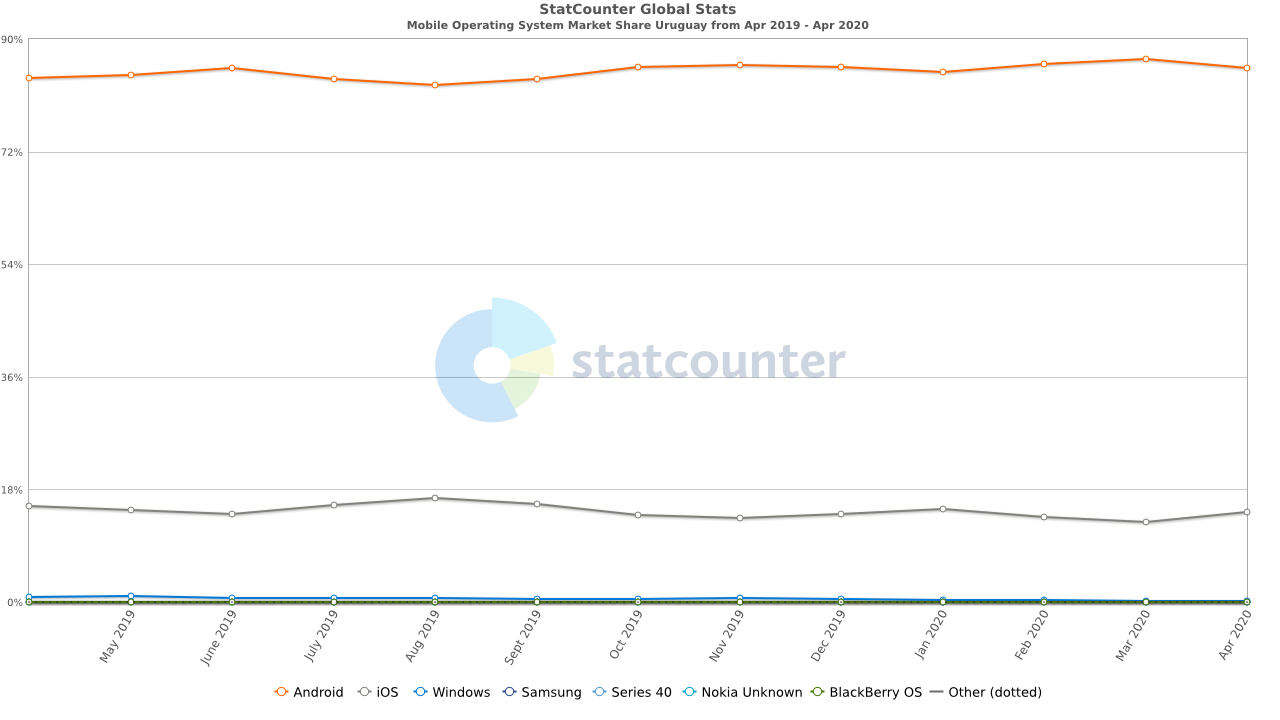
\includegraphics[width=\textwidth]{TESIS/imagenes/chap04/StatCounter-os_combined-UY-monthly-201904-202004.png}
\caption{ Sistemas operativos empleados en dispositivos móviles en Uruguay -periodo 04.2019 a 04.2020- \cite{StatCounter} }
\label{fig:uy-mobile-so}
\end{figure}

Con el objetivo de realizar un sistema más accesible para los usuarios, se decidió desarrollar la aplicación para la plataforma Android. Sin embargo, existen diversas tecnologías para el desarrollo de aplicaciones multiplataforma -que luego pueden ser soportadas por ambos sistemas operativos- (p.ej: Flutter, Xamarin, Genexus, etc.). Además, la comunidad de soporte para el uso del dispositivo de medición seleccionado existe para los lenguajes nativos de Android -Java o Kotlin-, lo que facilita la implementación y la solución de inconvenientes durante el desarrollo de la aplicación móvil, sobre todo para la interoperabilidad de la misma con el dispositivo de medición inercial.  

\section{Interfaz y experiencia de usuario (UI \& UX)}

% UX & UI 
En la última década, la ``experiencia de usuario'' (UX) se convirtió en una palabra de gran importancia en el campo de la interacción humano-computadora (HCI) y el diseño de interacción. A medida que la tecnología maduró, los productos interactivos se volvieron no solo más útiles y utilizables, sino también más modernos y fascinantes \cite{Hassenzahl2006}. Se puede decir entonces, que la experiencia de usuario no es nada más ni nada menos que cómo se siente el usuario al interactuar con un sistema de software. 

% Cualidades del software que se buscan con UI & UX 
En el área de desarrollo de aplicaciones móviles, la definición de la interfaz de usuario (UI) y la forma en que se va a interactuar con dicha aplicación es una etapa fundamental. El diseño de la interfaz de usuario debe tener en cuenta el público objetivo de dicha aplicación, para que el resultado final sea entendible y accesible para dicho público. 

% Material Design
Por lo tanto, a fin de generar un buen diseño de la interfaz de usuario (UI) se deben seguir los lineamientos de diseño que la plataforma sugiere, ya que el usuario de ese dispositivo estará familiarizado con dichos lineamientos. En este sentido, la plataforma Android ofrece una guía de diseño llamada ``Material Design'', utilizada por la gran mayoría de las aplicaciones disponibles en la plataforma. Material Design, es un conjunto de guías, componentes y herramientas que engloban las mejores practicas de diseño de UI para Android \cite{MaterialDesign}. 
 
% Sketch 
En PARKIBIP, se utilizó Material Design para diseñar tanto la interfaz de usuario como la experiencia de usuario. Para esto, se empleo la herramienta de diseño gráfico y prototipado Sketch (© 2020 Sketch B.V.). Sketch es un editor de vectores gráficos funcional en macOS, desarrollado por la empresa holandesa Boheamian Coding. Es utilizada para el diseño de UI y UX por más de un millón de usuarios en todo el mundo. Además, tiene funcionalidades para prototipado de aplicaciones y colaboración. 

\section{Especificación detallada y alcance del proyecto }
\label{chap:project-scope}

% Objetivo del producto
El presente proyecto tiene como objetivo la implementación de PARKIBIP, un sistema que le brinde soporte a la toma de decisiones de un terapeuta y a su vez, le permita a los pacientes con la enfermedad de Parkinson una rehabilitación personal. Durante las sesiones de fisioterapia los estímulos externos pueden mejorar las características de la marcha. PARKIBIP entonces busca emular estos estímulos en tiempo real para permitirle al enfermo una rehabilitación personal que prolongue el trabajo del fisioterapeuta en su vida cotidiana. Es decir, reeducar al paciente en rehabilitación mediante feedback -estímulos adecuados y repetitivos- a manipular eventos fisiológicos no detectados de forma voluntaria, logrando una función terapéutica.

Por lo tanto, integrando los avances en dispositivos de análisis de la marcha con los teléfonos inteligentes de uso cotidiano, haciendo uso de la evidencia adquirida a lo largo del tiempo en las terapias de Biofeedback para lograr construir un sistema portable -uso cotidiano y en exteriores-, accesible y de bajo costo; cuyo objetivo sea aumentar el control voluntario sobre los procesos fisiológicos. Mediante un dispositivo electrónico vestible de bajo costo (IMU - Unidad de Medición Inercial), que combina múltiples sensores (p. ej. acelerómetro, giroscopio, magnetómetro, entre otros), se particiona el ciclo de marcha del usuario permitiendo identificar distintos eventos, tales como, el contacto inicial con el suelo o la fase de vuelo. Finalmente, con los eventos detectados, se aplican ciertos algoritmos matemáticos que calculan los parámetros espacio temporales claves, y en base a un módulo clínico se estimula adecuadamente al usuario.

% Alcance
Definir el alcance del proyecto es una actividad central dentro del proceso de planeación del proyecto -también denominada ingeniería de requisitos-, que implica determinar y documentar una lista de objetivos finales, entregables y tareas específicas del proyecto. En otras palabras, es el trabajo a realizar, son las características y funcionalidades que caracterizan un producto, servicio o resultado; define los límites del proyecto, qué características se incluirán e implementarán dentro del mismo. 

En software, es habitual definir el alcance de un proyecto mediante la especificación de requisitos de software (SRS, del ingles Software Requirements Specification), siendo una descripción de un sistema a desarrollar. La SRS establece requisitos funcionales y no funcionales y en general incluye un conjunto de historias de usuario o casos de uso que el sistema debe proporcionar. 

% Historias de usuario
Una herramienta fundamental para definir el alcance de un trabajo es la historia de usuario, que debe ser completada para cumplir con los requisitos de una funcionalidad del producto o un objetivo del usuario de forma que la misma le brinde un valor particular. Es la unidad de trabajo más pequeña en un marco de desarrollo ágil y se encuentra expresado desde la perspectiva del usuario del software. Es decir, una historia de usuario es una explicación general e informal de una funcionalidad del sistema, escrita desde la perspectiva del usuario final en lenguaje natural. Asimismo, una Épica es una unidad de alto nivel que contiene o desglosa un conjunto de tareas más pequeñas (historias de usuario).

Por lo tanto, se optó por construir la especificación de PARKIBIP en base a la definición de historias de usuarios, y por consiguiente su conjunto es el alcance de la solución. Algunas de los beneficios adicionales contemplados para emplear esta metodología fueron:

\begin{itemize}
    \item Una lista de tareas pendientes mantiene al equipo centrado en tareas que deben completarse, sin embargo un conjunto de historias lo mantiene centrado en solucionar problemas para el usuario final.
    \item Con el objetivo definido en historias, el equipo puede colaborar para decidir cómo implementar la mejor solución, dividir las tareas y cumplir con dicho objetivo.
    \item Las historias fomentan que el equipo piense de forma crítica y creativa sobre cómo lograr mejor un objetivo.
    \item Con cada historia el equipo de desarrollo realiza pequeños incrementos hacia el producto final y disfruta pequeños logros, lo que aumenta la motivación.
\end{itemize}

A continuación, se lista el conjunto de historias de usuario de PARKIBIP junto a sus actores, épica, descripción y nombre descriptivo. Cabe resaltar que el hecho de incluir la Épica y su desglose en historias, permite especificar de forma adicional el WBS  (del ingles, Work Breakdown Structure) del proyecto PARKIBIP. La nomenclatura de especificación para cada historia de usuario es: Como $<Rol>$ se Desea $<Objetivo>$ Para $<Beneficio>$.

\begin{table}[H] 
\centering
\begin{tabular}{| p{2cm} | p{10cm} |}
\hline
Épica & Usuario\\ \hline
Nombre & Autenticación y manejo de Sesión\\ \hline
Actores & Terapeuta | Paciente\\ \hline
Descripción &  Como Terapeuta o Paciente previamente registrado se desea acceder al sistema PARKIBIP. Para esto ingresará sus credenciales de acceso y el sistema realizará la validación y autorización correspondiente.\\ \hline
\end{tabular}
\end{table}

\begin{table}[H] 
\centering
\begin{tabular}{|p{2cm} | p{10cm} |}
\hline
Épica & Usuario\\ \hline
Nombre & Gestión de Roles y Permisos de Usuarios\\ \hline
Actores & PARKIBIP\\ \hline
Descripción &  Como Sistema se quiere distinguir a los Usuarios por su Rol. PARKIBIP podrá determinar la información y las funcionalidades que le son permitidas según el Rol del usuario activo y sus autorizaciones asociadas.\\ \hline
\end{tabular}
\end{table}

\begin{table}[H] 
\centering
\begin{tabular}{| p{2cm} | p{10cm} |}
\hline
Épica & Usuario\\ \hline
Nombre & Visualización de Usuario activo discriminado por Rol\\ \hline
Actores & Terapeuta | Paciente\\ \hline
Descripción &  Como Terapeuta o Paciente se quiere visualizar su información de usuario en el Sistema.\\ \hline
\end{tabular}
\end{table}

\begin{table}[H] 
\centering
\begin{tabular}{| p{2cm} | p{10cm} |}
\hline
Épica & IMU\\ \hline
Nombre & Escaneo de dispositivos Bluetooth\\ \hline
Actores & Terapeuta | Paciente\\ \hline
Descripción & Como Terapeuta o Paciente se desea identificar los dispositivos IMU en su radio cercano, y así iniciar las configuraciones pertinentes para su uso.\\ \hline
\end{tabular}
\end{table}

\begin{table}[H] 
\centering
\begin{tabular}{| p{2cm} | p{10cm} |}
\hline
Épica & IMU\\ \hline
Nombre & Emparejamiento y sincronización de Dispositivo IMU\\ \hline
Actores & Terapeuta | Paciente\\ \hline
Descripción &  Como Terapeuta o Paciente se quiere emparejar un dispositivo IMU previamente escaneado por PARKIBIP, conforme a iniciar sesiones de rehabilitación.\\ \hline
\end{tabular}
\end{table}

\begin{table}[H] 
\centering
\begin{tabular}{| p{2cm} | p{10cm} |}
\hline
Épica & IMU\\ \hline
Nombre & Establecer sensor de color LED de luz\\ \hline
Actores & PARKIBIP\\ \hline
Descripción &  Como Sistema se desea configurar el indicador LED de luz de un dispositivo previamente conectado. De esta manera, se logra distinguir visualmente -en la interfaz gráfica y en el cuerpo del paciente- el dispositivo conectado a cuál extremidad.\\ \hline
\end{tabular}
\end{table}

\begin{table}[H] 
\centering
\begin{tabular}{| p{2cm} | p{10cm} |}
\hline
Épica & IMU\\ \hline
Nombre & Establecer la tasa de datos de salida y el rango de datos del Sensor Acelerómetro\\ \hline
Actores & PARKIBIP\\ \hline
Descripción & Como Sistema se quiere establecer la frecuencia en Hz de recolección de datos y el rango posible de datos para el sensor Acelerómetro de un IMU sincronizado.  \\ \hline
\end{tabular}
\end{table}

\begin{table}[H] 
\centering
\begin{tabular}{| p{2cm} | p{10cm} |}
\hline
Épica & IMU\\ \hline
Nombre & Establecer la tasa de datos de salida y el rango de datos del Sensor Giroscopio\\ \hline
Actores & PARKIBIP\\ \hline
Descripción & Como Sistema se quiere establecer la frecuencia en Hz de recolección de datos y el rango posible de datos para el sensor Giroscopio de un IMU sincronizado.\\ \hline
\end{tabular}
\end{table}

\begin{table}[H] 
\centering
\begin{tabular}{| p{2cm} | p{10cm} |}
\hline
Épica & IMU\\ \hline
Nombre & Establecer el rango de datos,  ruido, corriente media del Sensor Magnetómetro\\ \hline
Actores & PARKIBIP\\ \hline
Descripción & Como Sistema se quiere establecer la frecuencia en Hz de recolección de datos, el ruido y la corriente media para el sensor Magnetómetro de un IMU sincronizado.\\ \hline
\end{tabular}
\end{table}

\begin{table}[H] 
\centering
\begin{tabular}{| p{2cm} | p{10cm} |}
\hline
Épica & IMU\\ \hline
Nombre & Iniciar recolección asincónica de datos por sensor en un IMU\\ \hline
Actores & PARKIBIP\\ \hline
Descripción &  Como Sistema se quiere iniciar la recolección de datos crudos por tipo de sensor para un IMU previamente conectado. De acuerdo a las necesidades numéricas, el sistema será capaz de iniciar cada sensor correspondiente para un procesamiento posterior de datos.\\ \hline
\end{tabular} 
\end{table}

\begin{table}[H] 
\centering
\begin{tabular}{| p{2cm} | p{10cm} |}
\hline
Épica & IMU\\ \hline
Nombre & Detener recolección asincónica de datos por sensor en un IMU\\ \hline
Actores & PARKIBIP\\ \hline
Descripción &  Como Sistema se quiere detener la recolección de datos crudos por tipo de sensor para un sensor activo en un IMU previamente conectado. De esta manera, se liberan los recursos asignados en el IMU y en el Host para una posterior recolección.\\ \hline
\end{tabular}
\end{table}

\begin{table}[H] 
\centering
\begin{tabular}{| p{2cm} | p{10cm} |}
\hline
Épica & IMU\\ \hline
Nombre & Empaquetado de datos de múltiples sensores de un dispositivo IMU\\ \hline
Actores & PARKIBIP\\ \hline
Descripción & Como Sistema se quiere consolidar los diferentes datos recolectados (acelerómetro, giroscopio, magnetómetro) en un único paquete de datos con Timestamp de referencia. El requerimiento de manejar tantos threads como sensores activos, que a su vez tienen frecuencias distintas, incrementa la complejidad de empaquetado de datos. PARKIBIP debe implementar un algoritmo de empaquetado de datos consistente a las distintas frecuencias. \\ \hline
\end{tabular}
\end{table}

\begin{table}[H] 
\centering
\begin{tabular}{| p{2cm} | p{10cm} |}
\hline
Épica & IMU\\ \hline
Nombre & Administrar conexiones por dispositivo IMU\\ \hline
Actores & PARKIBIP\\ \hline
Descripción & Como Sistema se desea gestionar las diferentes conexiones a los múltiples dispositivos conectados, y así intercambiar distintos comandos con el IMU adecuado.\\ \hline
\end{tabular}
\end{table}

\begin{table}[H] 
\centering
\begin{tabular}{| p{2cm} | p{10cm} |}
\hline
Épica & IMU\\ \hline
Nombre & Establecer modulo de vibración IMU\\ \hline
Actores & PARKIBIP\\ \hline
Descripción &  Como Sistema se quiere configurar el motor vibratorio integrado al IMU, establecer la duración e intensidad de vibración. Siendo el presente modulo uno de los estímulos externos base a emplear en PARKIBIP.\\ \hline
\end{tabular}
\end{table}

\begin{table}[H] 
\centering
\begin{tabular}{| p{2cm} | p{10cm} |}
\hline
Épica & Configuración\\ \hline
Nombre & Visualización de parámetros y constantes Generales\\ \hline
Actores & Terapeuta | Paciente\\ \hline
Descripción & Como Terapeuta o Paciente se quiere visualizar parámetros generales de fabrica para evaluar dinámicamente su uso en una sesión de rehabilitación. \\ \hline
\end{tabular}
\end{table}

\begin{table}[H] 
\centering
\begin{tabular}{| p{2cm} | p{10cm} |}
\hline
Épica & Configuración\\ \hline
Nombre & Visualización de parámetros y constantes específicos por Método numérico\\ \hline
Actores & Terapeuta | Paciente\\ \hline
Descripción & Como Terapeuta o Paciente se quiere visualizar información de parámetros específicos por algoritmos.  \\ \hline
\end{tabular}
\end{table}

\begin{table}[H] 
\centering
\begin{tabular}{| p{2cm} | p{10cm} |}
\hline
Épica & Configuración\\ \hline
Nombre & Modificación de parámetros y constantes\\ \hline
Actores & Terapeuta | Paciente\\ \hline
Descripción & Como Terapeuta o Paciente se quiere actualizar parámetros generales y específicos de algoritmos. Permitiendo afinar el comportamiento del algoritmo elegido según las necesidades clínicas del paciente en rehabilitación. \\ \hline
\end{tabular}
\end{table}

\begin{table}[H] 
\centering
\begin{tabular}{| p{2cm} | p{10cm} |}
\hline
Épica & Configuración\\ \hline
Nombre & Restablecer valores de parámetros y constantes\\ \hline
Actores & Terapeuta | Paciente\\ \hline
Descripción & Como Terapeuta o Paciente se desea actualizar los parámetros generales y específicos de algoritmos a sus valores de fabrica elegidos como óptimos por los desarrolladores. \\ \hline
\end{tabular}
\end{table}

\begin{table}[H] 
\centering
\begin{tabular}{| p{2cm} | p{10cm} |}
\hline
Épica & Configuración\\ \hline
Nombre & Deshacer cambios de parámetros y constantes\\ \hline
Actores & Terapeuta | Paciente\\ \hline
Descripción & Como Terapeuta o Paciente se desea deshacer cambios involuntarios de parámetros, retornando a la configuración previa. \\ \hline
\end{tabular}
\end{table}

\begin{table}[H] 
\centering
\begin{tabular}{| p{2cm} | p{10cm} |}
\hline
Épica & Paciente\\ \hline
Nombre & Alta de Pacientes\\ \hline
Actores & Terapeuta\\ \hline
Descripción & Como Terapeuta se quiere dar de alta Pacientes para que puedan participar de sesiones de rehabilitación. \\ \hline
\end{tabular}
\end{table}

\begin{table}[H] 
\centering
\begin{tabular}{| p{2cm} | p{10cm} |}
\hline
Épica & Paciente\\ \hline
Nombre & Visualización y listado de Pacientes\\ \hline
Actores & Terapeuta\\ \hline
Descripción & Como Terapeuta se desea visualizar la plantilla de Pacientes junto a su información básica. \\ \hline
\end{tabular}
\end{table}

\begin{table}[H] 
\centering
\begin{tabular}{| p{2cm} | p{10cm} |}
\hline
Épica & Paciente\\ \hline
Nombre & Búsqueda y filtrado de Pacientes\\ \hline
Actores & Terapeuta\\ \hline
Descripción &  Como Terapeuta se desea buscar de forma amigable un Paciente mediante filtros conforme a seleccionarlo como usuario activo de Sesiones de rehabilitación.\\ \hline
\end{tabular}
\end{table}

\begin{table}[H] 
\centering
\begin{tabular}{| p{2cm} | p{10cm} |}
\hline
Épica & Paciente\\ \hline
Nombre & Selección de Paciente activo\\ \hline
Actores & Terapeuta\\ \hline
Descripción &  Como Terapeuta, visualizando el listado de Pacientes y haciendo uso del buscador, podrá establecer un Paciente como Usuario activo. El Sistema reconocerá automáticamente al Usuario activo como el participante de una Sesión de rehabilitación.\\ \hline
\end{tabular}
\end{table}

\begin{table}[H] 
\centering
\begin{tabular}{| p{2cm} | p{10cm} |}
\hline
Épica & Paciente\\ \hline
Nombre & Recuperación de último Estado de Sistema\\ \hline
Actores & PARKIBIP\\ \hline
Descripción &  Como Sistema se quiere facilitar y automatizar toda característica de Parkibip de forma que se minimice la selección/digitación por parte del usuario de PARKIBIP. Para ello, el Sistema mantendrá distintos Estados de la aplicación y será capaz de almacenar y recuperar su ultimo Estado (p. ej. Paciente activo, Usuario Logueado, Configuraciones, etc.) \\ \hline
\end{tabular}
\end{table}

\begin{table}[H] 
\centering
\begin{tabular}{| p{2cm} | p{10cm} |}
\hline
Épica & Sesión\\ \hline
Nombre & Visualización e Historial de Sesiones \\ \hline
Actores & Terapeuta | Paciente\\ \hline
Descripción & Como Terapeuta o Paciente se desea visualizar el Historial de Sesiones de rehabilitación ordenadas de forma descendente por cada fecha de realización. El listado permitirá ver información básica de la Sesión y navegar a su información mas detallada. \\ \hline
\end{tabular}
\end{table}

\begin{table}[H] 
\centering
\begin{tabular}{| p{2cm} | p{10cm} |}
\hline
Épica & Sesión\\ \hline
Nombre & Búsqueda y filtrado de Sesiones históricas\\ \hline
Actores & Terapeuta | Paciente\\ \hline
Descripción & Como Terapeuta o Paciente se desea buscar de forma amigable cada Sesión dentro del Historial de Sesiones mediante filtros, y así obtener información detallada según necesidad del usuario. \\ \hline
\end{tabular}
\end{table}

\begin{table}[H] 
\centering
\begin{tabular}{| p{2cm} | p{10cm} |}
\hline
Épica & Sesión\\ \hline
Nombre & Selección de Sesión\\ \hline
Actores & Terapeuta | Paciente \\ \hline
Descripción & Como Terapeuta o Paciente se quiere obtener información particular respecto a una Sesión previamente realizada. Para ello, mediante el uso del buscador podrá filtrar las sesiones de rehabilitación e ingresar a una interfaz que presente información genérica y otra con un nivel de entendimiento técnico.\\ \hline
\end{tabular}
\end{table}

\begin{table}[H] 
\centering
\begin{tabular}{| p{2cm} | p{10cm} |}
\hline
Épica & Sesión\\ \hline
Nombre & Resumen general de Sesión\\ \hline
Actores & Terapeuta | Paciente\\ \hline
Descripción & Como Terapeuta o Paciente se desea analizar y evaluar cada Sesión de rehabilitación mediante la visualización del comportamiento de los parámetros espacio-temporales de la marcha efectuada. Algunos parámetros son: duración, cadencia, velocidad promedio e instantánea, aceleración promedio e instantánea.\\ \hline
\end{tabular}
\end{table}

\begin{table}[H] 
\centering
\begin{tabular}{| p{2cm} | p{10cm} |}
\hline
Épica & Sesión\\ \hline
Nombre & Resumen gráfico de Sesión\\ \hline
Actores & Terapeuta | Paciente\\ \hline
Descripción & Como Terapeuta o Paciente se desea analizar y evaluar cada Sesión de rehabilitación de forma gráfica  respecto al tiempo (p. ej. velocidad, trayectoria, pasos).\\ \hline
\end{tabular}
\end{table}

\begin{table}[H] 
\centering
\begin{tabular}{| p{2cm} | p{10cm} |}
\hline
Épica & Sesión activa\\ \hline
Nombre & Iniciar Sesión de Rehabilitación\\ \hline
Actores & Terapeuta | Paciente \\ \hline
Descripción & Como Terapeuta o Paciente se quiere realizar una Sesión de rehabilitación para un Paciente activo. De esta forma, con las pre-condiciones funcionales cubiertas, el Sistema identificará las fases de la marcha y estimulará de acuerdo al protocolo pre-establecido. 

El usuario de PARKIBIP, únicamente tendrá que iniciar la Sesión, luego PARKIBIP automatizará por completo el flujo de proceso necesario para cumplir el requerimiento bajo el empleo de algoritmos numéricos particulares.

Algunas de las pre-condiciones son los dispositivos conectados, paciente activo seleccionado.\\ \hline
\end{tabular}
\end{table}

\begin{table}[H] 
\centering
\begin{tabular}{| p{2cm} | p{10cm} |}
\hline
Épica & Sesión activa\\ \hline
Nombre & Detener Sesión para Paciente activo\\ \hline
Actores & Terapeuta | Paciente\\ \hline
Descripción & Como Terapeuta o Paciente  se desea detener una Sesión de rehabilitación previamente iniciada. El Sistema liberará recursos asignados -rendimiento y consumo energético de dispositivos- y presentara una interfaz con los resultados detallados de la Sesión efectuada.\\ \hline
\end{tabular}
\end{table}

\begin{table}[H] 
\centering
\begin{tabular}{| p{2cm} | p{10cm} |}
\hline
Épica & Sesión activa\\ \hline
Nombre & Partición del ciclo de la marcha\\ \hline
Actores & PARKIBIP\\ \hline
Descripción & Como Sistema se quiere detectar eficazmente y en tiempo real los eventos asociados a la partición del ciclo de la marcha de cada Paciente (p. ej. HS, TO). Mediante la recolección de datos en tiempo real de los distintos sensores del IMU, y bajo el procesamiento de algoritmos numéricos particulares (existentes o propuestos) el sistema será capaz de detectar la partición del ciclo de la marcha. 

Para ello, serán requisitos los dispositivos conectados, los sensores asociados establecidos, los dispositivos posicionados en los tobillos del paciente mediante banda elástica y una Sesión de rehabilitación activa recolectando los datos de sensores inerciales.  \\ \hline
\end{tabular}
\end{table}

\begin{table}[H] 
\centering
\begin{tabular}{| p{2cm} | p{10cm} |}
\hline
Épica & Sesión activa\\ \hline
Nombre & Identificación adecuada de estímulos en base a procesamiento de reglas\\ \hline
Actores & PARKIBIP\\ \hline
Descripción & Como Sistema se quiere automatizar la identificación adecuada de estímulos, bajo el soporte de la funcionalidad Partición del ciclo de la marcha, para lograr estimular al Paciente en rehabilitación cuando corresponda. \\ \hline
\end{tabular}
\end{table}

\begin{table}[H] 
\centering
\begin{tabular}{| p{2cm} | p{10cm} |}
\hline
Épica & Sesión activa\\ \hline
Nombre & Estimular de forma vibratoria al Paciente de acuerdo a protocolo preestablecido\\ \hline
Actores & PARKIBIP\\ \hline
Descripción &  Como Sistema se desea estimular mediante vibración el cuerpo del Paciente en rehabilitación, que se encuentra unido al dispositivo IMU durante una Sesión activa. El estimulo externo, sera el feedback que reeduque la marcha del sujeto afectado. Para ello, PARKIBIP deberá implementar un Protocolo clínico que indique el instante de estimulación externa.\\ \hline
\end{tabular}
\end{table}

\begin{table}[H] 
\centering
\begin{tabular}{| p{2cm} | p{10cm} |}
\hline
Épica & Sesión activa\\ \hline
Nombre & Estimular de forma sonora al Paciente de acuerdo a protocolo preestablecido\\ \hline
Actores & PARKIBIP\\ \hline
Descripción &  Como Sistema se desea estimular de forma sonora al Paciente en rehabilitación durante una Sesión activa. Idéntico al estimulo vibratorio, PARKIBIP deberá empleará un Protocolo clínico que indique el instante de estimulación externa.\\ \hline
\end{tabular}
\end{table}

\begin{table}[H] 
\centering
\begin{tabular}{| p{2cm} | p{10cm} |}
\hline
Épica & Sesión activa\\ \hline
Nombre & Computo de parámetros espacio-temporales de interés\\ \hline
Actores & PARKIBIP\\ \hline
Descripción & Como Sistema se desea realizar una estimación en tiempo real de los parámetros espacio-temporales de la marcha durante una sesión de rehabilitación. Mediante la recolección de datos en tiempo real de los distintos sensores del IMU, y bajo el procesamiento de algoritmos numéricos particulares (existentes o propuestos), PARKIBIP será capaz de estimar la duración, la cadencia, la velocidad, la aceleración y la cantidad de pasos en el transcurso de la Sesión. Logrando un resumen objetivo de la marcha del sujeto afectado y siendo el soporte a toma de decisiones posteriores, que de otra forma serían subjetivas.\\ \hline
\end{tabular}
\end{table}

\begin{table}[H] 
\centering
\begin{tabular}{| p{2cm} | p{10cm} |}
\hline
Épica & Biofeedback\\ \hline
Nombre & Configuración de modo de estimulo: Vibratorio y/o sonoro\\ \hline
Actores & Terapeuta | Paciente\\ \hline
Descripción & Como Terapeuta o Paciente se quiere establecer el formato de estimulación externa al Paciente en rehabilitación; con el fin de maximizar resultados en el re-aprendizaje de una marcha adecuada. \\ \hline
\end{tabular}
\end{table}

\begin{table}[H] 
\centering
\begin{tabular}{| p{2cm} | p{10cm} |}
\hline
Épica & Biofeedback\\ \hline
Nombre & Modulo de Biofeedback. Configuración de Protocolo de estimulo\\ \hline
Actores & Terapeuta\\ \hline
Descripción &  Como Terapeuta se quiere establecer un formato condicional de estímulos, bajo el desarrollo de reglas clínicas de decisión. Según las necesidades del Paciente, el protocolo indica las necesidades de estímulos para dicho sujeto, indicando el instante temporal, característica disparadora, modo de estimulo. En otras palabras, el Protocolo PARKIBIP es análogo a una receta clínica. \\ \hline
\end{tabular}
\end{table}




